\documentclass[12pt,a4paper]{article}

% Packages
\usepackage{amsmath}
\usepackage{amssymb}
\usepackage{amsthm}
\usepackage[margin=1in]{geometry}
\usepackage{enumitem}
\usepackage{xcolor}
\usepackage{mathtools}
\usepackage{tikz}

% Custom environments
\newtheorem{explanation}{Explanation}
\theoremstyle{definition}
\newtheorem{solution}{Solution}

% Custom commands
\newcommand{\stage}[1]{\textbf{\textcolor{blue}{#1}}}

% Title information
\title{Methods of Applied Mathematics - Part 1\\
Exercise Sheet 2: Question 3\\
Stability in 2D Systems}
\author{Complete Solution with XYZ Methodology}
\date{}

\begin{document}

\maketitle

\section*{Problem Statement}

Consider the 2D ODE:
\begin{align}
\dot{x} &= x - 4y \\
\dot{y} &= y - x
\end{align}
with initial condition $x(0) = 1, y(0) = 0$.

\section{Question 3(a): Equilibria, Stability, and Classification}

\begin{solution}

\subsection*{Step 1: Find the Equilibria}

\begin{itemize}[leftmargin=*]
\item \stage{STAGE X (What we need):} An equilibrium $(x^*, y^*)$ is a point where the system doesn't change, i.e., where $\dot{x} = 0$ and $\dot{y} = 0$ simultaneously.

\item \stage{STAGE Y (Why this approach):} From Lecture Notes (Section 6, page 21), equilibria of a system $\dot{\mathbf{x}} = \mathbf{f}(\mathbf{x})$ occur where $\mathbf{f}(\mathbf{x}^*) = \mathbf{0}$. For our 2D system, we solve the coupled algebraic equations.

\item \stage{STAGE Z (What we'll do):} Set both equations to zero and solve for $(x^*, y^*)$.
\end{itemize}

\textbf{Step 1A: Set Up the Equilibrium Equations}

\begin{align}
\dot{x} = 0 &\quad \Rightarrow \quad x - 4y = 0 \\
\dot{y} = 0 &\quad \Rightarrow \quad y - x = 0
\end{align}

\textbf{Step 1B: Solve the System}

From the second equation:
\begin{equation}
y - x = 0 \quad \Rightarrow \quad y = x
\end{equation}

Substitute into the first equation:
\begin{align}
x - 4y &= 0 \\
x - 4x &= 0 \\
-3x &= 0 \\
x &= 0
\end{align}

Therefore: $x = 0$ and $y = 0$.

\begin{equation}
\boxed{\text{Unique equilibrium: } (x^*, y^*) = (0, 0)}
\end{equation}

\begin{explanation}[Verification]
Check by substitution:
\begin{align}
\dot{x}\big|_{(0,0)} &= 0 - 4(0) = 0 \quad \checkmark \\
\dot{y}\big|_{(0,0)} &= 0 - 0 = 0 \quad \checkmark
\end{align}
\end{explanation}

\subsection*{Step 2: Write System in Matrix Form}

To analyze stability, we write the system in matrix-vector form.

The system is already linear:
\begin{equation}
\begin{pmatrix} \dot{x} \\ \dot{y} \end{pmatrix} =
\begin{pmatrix} 1 & -4 \\ -1 & 1 \end{pmatrix}
\begin{pmatrix} x \\ y \end{pmatrix}
\end{equation}

So we have $\dot{\mathbf{x}} = A\mathbf{x}$ where:
\begin{equation}
A = \begin{pmatrix} 1 & -4 \\ -1 & 1 \end{pmatrix}
\end{equation}

\begin{explanation}[Why Matrix Form Matters]
From Lecture Notes (Section 7, page 24): For a linear system $\dot{\mathbf{x}} = A\mathbf{x}$, the solution is $\mathbf{x}(t) = e^{At}\mathbf{x}_0$. The behavior near equilibrium is completely determined by the eigenvalues and eigenvectors of the matrix $A$.

For a general nonlinear system, we would compute the Jacobian matrix at the equilibrium. Here, the system is already linear, so $A$ is exactly the Jacobian everywhere.
\end{explanation}

\subsection*{Step 3: Compute Eigenvalues}

\begin{itemize}[leftmargin=*]
\item \stage{STAGE X (What eigenvalues tell us):} From Lecture Notes (Section 8, pages 29-31), eigenvalues determine stability and equilibrium type:
\begin{itemize}
\item Sign of real parts $\Rightarrow$ stable or unstable
\item Real vs. complex $\Rightarrow$ node/saddle vs. focus/center
\end{itemize}

\item \stage{STAGE Y (How to find them):} Solve the characteristic equation $\det(A - \lambda I) = 0$.

\item \stage{STAGE Z (What we expect):} Two eigenvalues $\lambda_1, \lambda_2$ (possibly complex conjugates).
\end{itemize}

\textbf{Step 3A: Set Up Characteristic Equation}

\begin{equation}
\det(A - \lambda I) = \det\begin{pmatrix} 1-\lambda & -4 \\ -1 & 1-\lambda \end{pmatrix} = 0
\end{equation}

\textbf{Step 3B: Compute the Determinant}

\begin{align}
\det(A - \lambda I) &= (1-\lambda)(1-\lambda) - (-4)(-1) \\
&= (1-\lambda)^2 - 4 \\
&= 1 - 2\lambda + \lambda^2 - 4 \\
&= \lambda^2 - 2\lambda - 3
\end{align}

\textbf{Step 3C: Solve the Characteristic Equation}

\begin{align}
\lambda^2 - 2\lambda - 3 &= 0
\end{align}

Using the quadratic formula:
\begin{align}
\lambda &= \frac{2 \pm \sqrt{4 + 12}}{2} \\
&= \frac{2 \pm \sqrt{16}}{2} \\
&= \frac{2 \pm 4}{2}
\end{align}

Therefore:
\begin{align}
\lambda_1 &= \frac{2 + 4}{2} = 3 \\
\lambda_2 &= \frac{2 - 4}{2} = -1
\end{align}

\begin{equation}
\boxed{\text{Eigenvalues: } \lambda_1 = 3, \quad \lambda_2 = -1}
\end{equation}

\subsection*{Step 4: Determine Stability}

\begin{explanation}[Stability Criterion from Lecture Notes (Section 8, page 29)]
For a 2D linear system with eigenvalues $\lambda_1, \lambda_2$:
\begin{itemize}
\item \textbf{Stable}: Both $\text{Re}(\lambda_1) < 0$ and $\text{Re}(\lambda_2) < 0$
\item \textbf{Unstable}: At least one $\text{Re}(\lambda_i) > 0$
\item \textbf{Saddle}: One positive, one negative real eigenvalue
\end{itemize}
\end{explanation}

Analysis of our eigenvalues:
\begin{itemize}
\item $\lambda_1 = 3 > 0$ (positive, real)
\item $\lambda_2 = -1 < 0$ (negative, real)
\end{itemize}

Since we have one positive and one negative eigenvalue:

\begin{equation}
\boxed{\text{The equilibrium is a \textbf{SADDLE} (unstable)}}
\end{equation}

\subsection*{Step 5: Classify the Equilibrium Type}

From Lecture Notes (Section 8, pages 29-31), classification scheme:

\begin{center}
\begin{tabular}{|l|l|l|}
\hline
\textbf{Eigenvalue Type} & \textbf{Signs} & \textbf{Classification} \\
\hline
Both real, same sign & $\lambda_1, \lambda_2 > 0$ & Unstable node \\
Both real, same sign & $\lambda_1, \lambda_2 < 0$ & Stable node \\
Both real, opposite signs & $\lambda_1 > 0, \lambda_2 < 0$ & \textbf{Saddle} \\
Complex conjugates & $\text{Re}(\lambda) > 0$ & Unstable focus/spiral \\
Complex conjugates & $\text{Re}(\lambda) < 0$ & Stable focus/spiral \\
Pure imaginary & $\text{Re}(\lambda) = 0$ & Center \\
\hline
\end{tabular}
\end{center}

Our case: $\lambda_1 = 3 > 0$ and $\lambda_2 = -1 < 0$ (both real, opposite signs)

\begin{equation}
\boxed{\text{Classification: \textbf{SADDLE POINT}}}
\end{equation}

\begin{explanation}[Physical Meaning of a Saddle]
\textbf{Behavior near the equilibrium:}
\begin{itemize}
\item Along the \textbf{unstable eigendirection} (associated with $\lambda_1 = 3$): trajectories are repelled exponentially with rate $e^{3t}$
\item Along the \textbf{stable eigendirection} (associated with $\lambda_2 = -1$): trajectories are attracted exponentially with rate $e^{-t}$
\end{itemize}

\textbf{Global behavior:}
\begin{itemize}
\item Most trajectories are repelled (because $|\lambda_1| > |\lambda_2|$, unstable direction dominates)
\item Only trajectories starting exactly on the stable manifold approach the saddle
\item The saddle is overall unstable
\end{itemize}
\end{explanation}

\subsection*{Step 6: Compute Eigenvectors (for Part b)}

To fully characterize the saddle and for solving in part (b), we need the eigenvectors.

\textbf{Step 6A: Eigenvector for $\lambda_1 = 3$}

Solve $(A - 3I)\mathbf{v}_1 = \mathbf{0}$:
\begin{equation}
\begin{pmatrix} 1-3 & -4 \\ -1 & 1-3 \end{pmatrix}
\begin{pmatrix} v_{1x} \\ v_{1y} \end{pmatrix} =
\begin{pmatrix} -2 & -4 \\ -1 & -2 \end{pmatrix}
\begin{pmatrix} v_{1x} \\ v_{1y} \end{pmatrix} =
\begin{pmatrix} 0 \\ 0 \end{pmatrix}
\end{equation}

First row: $-2v_{1x} - 4v_{1y} = 0 \Rightarrow v_{1x} = -2v_{1y}$

Choose $v_{1y} = 1$, then $v_{1x} = -2$:
\begin{equation}
\mathbf{v}_1 = \begin{pmatrix} -2 \\ 1 \end{pmatrix} \quad \text{or normalized: } \mathbf{c}_1 = \begin{pmatrix} 2 \\ -1 \end{pmatrix}
\end{equation}

\textbf{Step 6B: Eigenvector for $\lambda_2 = -1$}

Solve $(A + I)\mathbf{v}_2 = \mathbf{0}$:
\begin{equation}
\begin{pmatrix} 1+1 & -4 \\ -1 & 1+1 \end{pmatrix}
\begin{pmatrix} v_{2x} \\ v_{2y} \end{pmatrix} =
\begin{pmatrix} 2 & -4 \\ -1 & 2 \end{pmatrix}
\begin{pmatrix} v_{2x} \\ v_{2y} \end{pmatrix} =
\begin{pmatrix} 0 \\ 0 \end{pmatrix}
\end{equation}

First row: $2v_{2x} - 4v_{2y} = 0 \Rightarrow v_{2x} = 2v_{2y}$

Choose $v_{2y} = 1$, then $v_{2x} = 2$:
\begin{equation}
\mathbf{v}_2 = \mathbf{c}_2 = \begin{pmatrix} 2 \\ 1 \end{pmatrix}
\end{equation}

\textbf{Verification:}
\begin{align}
A\mathbf{v}_1 &= \begin{pmatrix} 1 & -4 \\ -1 & 1 \end{pmatrix}\begin{pmatrix} 2 \\ -1 \end{pmatrix} = \begin{pmatrix} 2+4 \\ -2-1 \end{pmatrix} = \begin{pmatrix} 6 \\ -3 \end{pmatrix} = 3\begin{pmatrix} 2 \\ -1 \end{pmatrix} \quad \checkmark \\
A\mathbf{v}_2 &= \begin{pmatrix} 1 & -4 \\ -1 & 1 \end{pmatrix}\begin{pmatrix} 2 \\ 1 \end{pmatrix} = \begin{pmatrix} 2-4 \\ -2+1 \end{pmatrix} = \begin{pmatrix} -2 \\ -1 \end{pmatrix} = -1\begin{pmatrix} 2 \\ 1 \end{pmatrix} \quad \checkmark
\end{align}

\subsection*{Step 7: Characterize Stable and Unstable Manifolds}

From Lecture Notes (Section 10, pages 34-35):

\begin{itemize}
\item \textbf{Unstable manifold} $W^u(0,0)$: The set of points approaching $(0,0)$ as $t \to -\infty$.
\begin{equation}
W^u(0,0) = \text{span}\{\mathbf{v}_1\} = \left\{c\begin{pmatrix} 2 \\ -1 \end{pmatrix} : c \in \mathbb{R}\right\}
\end{equation}
This is the line $y = -\frac{1}{2}x$ through the origin.

\item \textbf{Stable manifold} $W^s(0,0)$: The set of points approaching $(0,0)$ as $t \to +\infty$.
\begin{equation}
W^s(0,0) = \text{span}\{\mathbf{v}_2\} = \left\{c\begin{pmatrix} 2 \\ 1 \end{pmatrix} : c \in \mathbb{R}\right\}
\end{equation}
This is the line $y = \frac{1}{2}x$ through the origin.
\end{itemize}

\subsection*{Final Answer for Part (a)}

\begin{equation}
\boxed{
\begin{aligned}
&\textbf{Equilibrium: } (x^*, y^*) = (0, 0) \text{ (unique)} \\
&\textbf{Eigenvalues: } \lambda_1 = 3 \text{ (unstable)}, \quad \lambda_2 = -1 \text{ (stable)} \\
&\textbf{Eigenvectors: } \mathbf{c}_1 = \begin{pmatrix} 2 \\ -1 \end{pmatrix}, \quad \mathbf{c}_2 = \begin{pmatrix} 2 \\ 1 \end{pmatrix} \\
&\textbf{Type: SADDLE POINT (unstable)} \\
&\textbf{Stable manifold: } y = \frac{1}{2}x \quad (\text{along } \mathbf{c}_2) \\
&\textbf{Unstable manifold: } y = -\frac{1}{2}x \quad (\text{along } \mathbf{c}_1)
\end{aligned}
}
\end{equation}

\end{solution}

\vspace{10pt}
\hrule
\vspace{10pt}

\section{Question 3(b): Solve the System and Verify}

\begin{solution}

\subsection*{Step 1: General Solution Form via Eigendecomposition}

\begin{itemize}[leftmargin=*]
\item \stage{STAGE X (What we know):} From Lecture Notes (Section 7, page 28, equation 7.12), for a linear system $\dot{\mathbf{x}} = A\mathbf{x}$ with eigenvalues $\lambda_1, \lambda_2$ and eigenvectors $\mathbf{c}_1, \mathbf{c}_2$, the general solution is:
\begin{equation}
\mathbf{x}(t) = \alpha_1 \mathbf{c}_1 e^{\lambda_1 t} + \alpha_2 \mathbf{c}_2 e^{\lambda_2 t}
\end{equation}

\item \stage{STAGE Y (Why this works):} Each eigenvector gives an independent solution. Along eigenvector $\mathbf{c}_i$, the system behaves like a 1D exponential with rate $\lambda_i$. The general solution is a linear combination of these two fundamental solutions.

\item \stage{STAGE Z (Our task):} Substitute our eigenvalues and eigenvectors, then use initial conditions to find $\alpha_1$ and $\alpha_2$.
\end{itemize}

\subsection*{Step 2: Write the General Solution}

From part (a):
\begin{itemize}
\item $\lambda_1 = 3$, $\mathbf{c}_1 = \begin{pmatrix} 2 \\ -1 \end{pmatrix}$
\item $\lambda_2 = -1$, $\mathbf{c}_2 = \begin{pmatrix} 2 \\ 1 \end{pmatrix}$
\end{itemize}

General solution:
\begin{equation}
\begin{pmatrix} x(t) \\ y(t) \end{pmatrix} =
\alpha_1 \begin{pmatrix} 2 \\ -1 \end{pmatrix} e^{3t} +
\alpha_2 \begin{pmatrix} 2 \\ 1 \end{pmatrix} e^{-t}
\end{equation}

In component form:
\begin{align}
x(t) &= 2\alpha_1 e^{3t} + 2\alpha_2 e^{-t} \\
y(t) &= -\alpha_1 e^{3t} + \alpha_2 e^{-t}
\end{align}

\subsection*{Step 3: Apply Initial Conditions}

Given: $x(0) = 1$ and $y(0) = 0$

At $t = 0$:
\begin{align}
x(0) &= 2\alpha_1 e^{0} + 2\alpha_2 e^{0} = 2\alpha_1 + 2\alpha_2 = 1 \\
y(0) &= -\alpha_1 e^{0} + \alpha_2 e^{0} = -\alpha_1 + \alpha_2 = 0
\end{align}

This gives us the system:
\begin{align}
2\alpha_1 + 2\alpha_2 &= 1 \\
-\alpha_1 + \alpha_2 &= 0
\end{align}

\textbf{Step 3A: Solve for $\alpha_1$ and $\alpha_2$}

From the second equation:
\begin{equation}
\alpha_2 = \alpha_1
\end{equation}

Substitute into the first equation:
\begin{align}
2\alpha_1 + 2\alpha_1 &= 1 \\
4\alpha_1 &= 1 \\
\alpha_1 &= \frac{1}{4}
\end{align}

Therefore:
\begin{equation}
\alpha_2 = \alpha_1 = \frac{1}{4}
\end{equation}

\begin{equation}
\boxed{\alpha_1 = \frac{1}{4}, \quad \alpha_2 = \frac{1}{4}}
\end{equation}

\subsection*{Step 4: Write the Particular Solution}

Substituting $\alpha_1 = \alpha_2 = \frac{1}{4}$ into the general solution:

\begin{equation}
\begin{pmatrix} x(t) \\ y(t) \end{pmatrix} =
\frac{1}{4} \begin{pmatrix} 2 \\ -1 \end{pmatrix} e^{3t} +
\frac{1}{4} \begin{pmatrix} 2 \\ 1 \end{pmatrix} e^{-t}
\end{equation}

In component form:
\begin{align}
x(t) &= \frac{1}{4}(2e^{3t} + 2e^{-t}) = \frac{1}{2}(e^{3t} + e^{-t}) \\
y(t) &= \frac{1}{4}(-e^{3t} + e^{-t}) = \frac{1}{4}(e^{-t} - e^{3t})
\end{align}

\begin{equation}
\boxed{
\begin{aligned}
x(t) &= \frac{1}{2}(e^{3t} + e^{-t}) \\
y(t) &= \frac{1}{4}(e^{-t} - e^{3t})
\end{aligned}
}
\end{equation}

\subsection*{Step 5: Verify the Solution (ESSENTIAL)}

We must verify that our solution satisfies:
\begin{enumerate}
\item The original ODEs
\item The initial conditions
\end{enumerate}

\textbf{Step 5A: Verify Initial Conditions}

\begin{align}
x(0) &= \frac{1}{2}(e^{0} + e^{0}) = \frac{1}{2}(1 + 1) = 1 \quad \checkmark \\
y(0) &= \frac{1}{4}(e^{0} - e^{0}) = \frac{1}{4}(1 - 1) = 0 \quad \checkmark
\end{align}

\textbf{Step 5B: Verify the ODEs}

Compute $\dot{x}(t)$:
\begin{align}
\dot{x}(t) &= \frac{d}{dt}\left[\frac{1}{2}(e^{3t} + e^{-t})\right] \\
&= \frac{1}{2}(3e^{3t} - e^{-t})
\end{align}

Compute $\dot{y}(t)$:
\begin{align}
\dot{y}(t) &= \frac{d}{dt}\left[\frac{1}{4}(e^{-t} - e^{3t})\right] \\
&= \frac{1}{4}(-e^{-t} - 3e^{3t})
\end{align}

Now check the first ODE: $\dot{x} = x - 4y$

Right-hand side:
\begin{align}
x - 4y &= \frac{1}{2}(e^{3t} + e^{-t}) - 4 \cdot \frac{1}{4}(e^{-t} - e^{3t}) \\
&= \frac{1}{2}(e^{3t} + e^{-t}) - (e^{-t} - e^{3t}) \\
&= \frac{1}{2}e^{3t} + \frac{1}{2}e^{-t} - e^{-t} + e^{3t} \\
&= \frac{3}{2}e^{3t} - \frac{1}{2}e^{-t} \\
&= \frac{1}{2}(3e^{3t} - e^{-t}) = \dot{x} \quad \checkmark
\end{align}

Check the second ODE: $\dot{y} = y - x$

Right-hand side:
\begin{align}
y - x &= \frac{1}{4}(e^{-t} - e^{3t}) - \frac{1}{2}(e^{3t} + e^{-t}) \\
&= \frac{1}{4}e^{-t} - \frac{1}{4}e^{3t} - \frac{1}{2}e^{3t} - \frac{1}{2}e^{-t} \\
&= -\frac{1}{4}e^{-t} - \frac{3}{4}e^{3t} \\
&= \frac{1}{4}(-e^{-t} - 3e^{3t}) = \dot{y} \quad \checkmark
\end{align}

Both ODEs are satisfied!

\subsection*{Step 6: Analyze Long-Term Behavior}

\begin{itemize}[leftmargin=*]
\item \stage{STAGE X (What happens as $t \to \infty$):} The solution contains $e^{3t}$ (growing) and $e^{-t}$ (decaying) terms.

\item \stage{STAGE Y (Why $e^{3t}$ dominates):} As $t \to \infty$, $e^{3t} \to \infty$ much faster than $e^{-t} \to 0$. The unstable mode dominates.

\item \stage{STAGE Z (What this means):} The trajectory is repelled from the saddle point along the unstable manifold direction.
\end{itemize}

\textbf{Asymptotic Behavior as $t \to \infty$:}

\begin{align}
x(t) &= \frac{1}{2}(e^{3t} + e^{-t}) \sim \frac{1}{2}e^{3t} \\
y(t) &= \frac{1}{4}(e^{-t} - e^{3t}) \sim -\frac{1}{4}e^{3t}
\end{align}

The ratio:
\begin{equation}
\frac{y(t)}{x(t)} \sim \frac{-\frac{1}{4}e^{3t}}{\frac{1}{2}e^{3t}} = -\frac{1}{2}
\end{equation}

This means the trajectory asymptotically approaches the line $y = -\frac{1}{2}x$, which is exactly the \textbf{unstable manifold} we found in part (a)!

\begin{equation}
\boxed{\text{As } t \to \infty: \quad (x(t), y(t)) \to \infty \text{ along the line } y = -\frac{1}{2}x}
\end{equation}

\textbf{Asymptotic Behavior as $t \to -\infty$:}

For large negative $t$, $e^{3t} \to 0$ and $e^{-t} \to \infty$:

\begin{align}
x(t) &\sim \frac{1}{2}e^{-t} \\
y(t) &\sim \frac{1}{4}e^{-t}
\end{align}

The ratio:
\begin{equation}
\frac{y(t)}{x(t)} \sim \frac{\frac{1}{4}e^{-t}}{\frac{1}{2}e^{-t}} = \frac{1}{2}
\end{equation}

This means as we go backward in time, the trajectory came from the line $y = \frac{1}{2}x$, which is the \textbf{stable manifold}!

\begin{equation}
\boxed{\text{As } t \to -\infty: \quad (x(t), y(t)) \to \infty \text{ along the line } y = \frac{1}{2}x}
\end{equation}

\subsection*{Step 7: Geometric Interpretation}

\begin{explanation}[Trajectory Behavior Confirms Saddle Structure]
\textbf{The solution verifies our part (a) analysis:}

\begin{enumerate}
\item \textbf{Starting point}: $(1, 0)$ does NOT lie on either eigendirection, so the trajectory is a mixture of both modes.

\item \textbf{Initial direction}: At $t = 0$, both exponentials contribute. Since $\alpha_1 = \alpha_2 = 1/4$, the trajectory initially combines both stable and unstable components.

\item \textbf{Forward evolution} ($t > 0$): The unstable mode $e^{3t}$ grows rapidly, dominating the solution. The trajectory is repelled from the origin along the unstable manifold direction $y = -\frac{1}{2}x$.

\item \textbf{Backward evolution} ($t < 0$): The stable mode $e^{-t}$ dominates (since $e^{-t}$ grows as we go backward in time). The trajectory approaches the origin from the stable manifold direction $y = \frac{1}{2}x$.

\item \textbf{Saddle geometry}: The trajectory forms a hyperbolic path, approaching the stable manifold in the past and departing along the unstable manifold in the future.
\end{enumerate}

This is the characteristic behavior of a saddle point.
\end{explanation}

\subsection*{Step 8: Sketch the Phase Portrait (Qualitative)}

\begin{center}
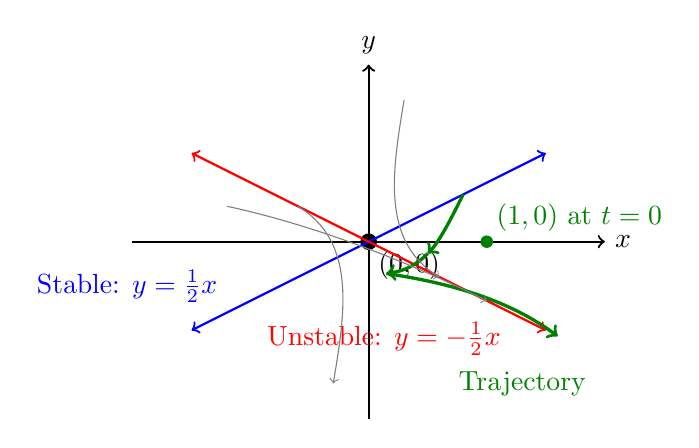
\begin{tikzpicture}[scale=1.5]
% Axes
\draw[->, thick] (-2,0) -- (2,0) node[right] {$x$};
\draw[->, thick] (0,-1.5) -- (0,1.5) node[above] {$y$};

% Origin (saddle point)
\fill (0,0) circle (2pt) node[below right] {$(0,0)$};

% Stable manifold: y = (1/2)x
\draw[blue, thick, <-] (-1.5,-0.75) -- (0,0);
\draw[blue, thick, ->] (0,0) -- (1.5,0.75);
\node[blue, above left] at (-1.2,-0.6) {Stable: $y=\frac{1}{2}x$};

% Unstable manifold: y = -(1/2)x
\draw[red, thick, ->] (0,0) -- (1.5,-0.75);
\draw[red, thick, <-] (-1.5,0.75) -- (0,0);
\node[red, below left] at (1.2,-0.6) {Unstable: $y=-\frac{1}{2}x$};

% Particular trajectory
\draw[green!50!black, very thick, ->] (0.8,0.4) .. controls (0.7,0.2) and (0.6,0) .. (0.5,-0.1);
\draw[green!50!black, very thick, ->] (0.5,-0.1) .. controls (0.4,-0.2) and (0.3,-0.25) .. (0.15,-0.27);
\draw[green!50!black, very thick, ->] (0.15,-0.27) .. controls (0.7,-0.35) and (1.2,-0.5) .. (1.6,-0.8);
\fill[green!50!black] (1,0) circle (1.5pt) node[above right] {$(1,0)$ at $t=0$};
\node[green!50!black] at (1.3,-1.2) {Trajectory};

% Other trajectories (qualitative)
\draw[gray, ->] (-1.2,0.3) .. controls (-0.5,0.15) and (0.3,-0.15) .. (1,-0.5);
\draw[gray, ->] (0.3,1.2) .. controls (0.2,0.6) and (0.1,0) .. (0.6,-0.3);
\draw[gray, <-] (-0.3,-1.2) .. controls (-0.2,-0.6) and (-0.1,0) .. (-0.6,0.3);
\end{tikzpicture}
\end{center}

\subsection*{Final Answer for Part (b)}

\begin{equation}
\boxed{
\begin{aligned}
&\textbf{Particular Solution:} \\
&x(t) = \frac{1}{2}(e^{3t} + e^{-t}) \\
&y(t) = \frac{1}{4}(e^{-t} - e^{3t}) \\[10pt]
&\textbf{Verification of Part (a):} \\
&\text{1. As } t \to \infty: \text{ trajectory escapes to } \infty \text{ along unstable manifold } y = -\frac{1}{2}x \\
&\text{2. As } t \to -\infty: \text{ trajectory came from stable manifold } y = \frac{1}{2}x \\
&\text{3. Trajectory is repelled from saddle (confirms unstable equilibrium)} \\
&\text{4. Solution exhibits characteristic saddle behavior: } \\
&\quad \text{mixture of } e^{3t} \text{ (unstable, grows) and } e^{-t} \text{ (stable, decays)}
\end{aligned}
}
\end{equation}

\end{solution}

\vspace{10pt}
\hrule
\vspace{10pt}

\section*{Summary: Complete Analysis of the 2D System}

\subsection*{Key Results}

\begin{enumerate}[leftmargin=*]
\item \textbf{Equilibrium}: $(0,0)$ is the unique equilibrium

\item \textbf{Matrix form}: $\dot{\mathbf{x}} = A\mathbf{x}$ where $A = \begin{pmatrix} 1 & -4 \\ -1 & 1 \end{pmatrix}$

\item \textbf{Eigenvalues}: $\lambda_1 = 3$ (unstable), $\lambda_2 = -1$ (stable)

\item \textbf{Eigenvectors}:
\begin{itemize}
\item $\mathbf{c}_1 = \begin{pmatrix} 2 \\ -1 \end{pmatrix}$ (unstable direction)
\item $\mathbf{c}_2 = \begin{pmatrix} 2 \\ 1 \end{pmatrix}$ (stable direction)
\end{itemize}

\item \textbf{Classification}: SADDLE POINT (unstable)

\item \textbf{Manifolds}:
\begin{itemize}
\item Stable: $y = \frac{1}{2}x$
\item Unstable: $y = -\frac{1}{2}x$
\end{itemize}

\item \textbf{Solution}: $x(t) = \frac{1}{2}(e^{3t} + e^{-t})$, $y(t) = \frac{1}{4}(e^{-t} - e^{3t})$

\item \textbf{Trajectory behavior}: Starts at $(1,0)$, initially moves toward origin along stable component, then rapidly repelled along unstable manifold toward infinity
\end{enumerate}

\subsection*{Connection to Lecture Notes}

This problem exemplifies the complete theory from Sections 7-8 of the lecture notes:
\begin{itemize}
\item \textbf{Eigendecomposition} (Section 7): Solution is a linear combination of eigenmodes
\item \textbf{Stability classification} (Section 8): Eigenvalue signs determine stability and type
\item \textbf{Stable/unstable manifolds} (Section 10): Eigenvectors define invariant manifolds
\item \textbf{Linear theory is exact}: For linear systems, the linearization IS the full dynamics
\end{itemize}

\end{document}
